Consideremos un sistema de ecuaciones diferenciales ordinarias (EDO) descrito por 
\begin{equation}
\dot{\mathbf{x}}(t) = f(\mathbf{x}(t),t)
\label{eq:ode}
\end{equation}
con $t$ el parametro que describe la evolución del sistema y $\flowci$ la trayectoria de la solución que en $t_0$ se encuentra en $\xo$. En la mayoría de los sistemas físicos, el parámetro $t$ describe al tiempo, ie, $t \in \mathbb{R}^+$, y al sistema de ODE se le conoce como sistema dinámico.

Pocos son los casos en donde la solución a $\dot{\mathbf{x}}(t)$ se puede obtener de manera analítica y, por tanto, estudiar las familias de soluciones para diferentes condiciones iniciales termina siendo, casi siempre, un estudio indirecto o aproximado. Se han enfrentado varias formas para darle la vuelta a este problema y, en los esfuerzos de lo aproximado, una de las soluciones más prácticas ha sido discretizar al parámetro temporal $t$ de (\ref{eq:ode}) y encontrar, en saltos discretos de $t$, el ``estado actual'' del sistema dado un ``estado anterior''.

Gracias a que hoy en día existe poder de cómputo para hacer muchas operaciones simples en relativamente poco tiempo, se ha explotado el estudio y uso de métodos iterativos para obtener $\flowci$, siendo de gran utilidad en los últimos años. Éstos se conocen como \textbf{métodos numéricos de integración de ecuaciones diferenciales}. Con estos métodos se puede, en la mayoría de los casos, definir una condición inicial $\xo := \mathbf{x}(t_0)$ y obtener la solución para esta condición particular. Sin embargo, no siempre es suficiente obtener la solución de una única condición inicial dada y, muchas veces, interesa todo una familia de soluciones alrededor de un punto $\xo$ de interés. Esto puede pasar, por ejemplo, en aceleradores de partículas que disparan paquetes de onda como si fuesen ``gotas" sujetas a algún campo externo. En mecánica de fluidos es interesante estudiar parcelas de fluidos y, con la representación lagranjiana de las ecuaciones de Navier-Stokes, ver cómo evolucionan estas parcelas en el tiempo; esta es una rama muy utilizada por los métodos computacionales, ya que por las no linealidades de las ecuaciones de Navier-Stokes, ha sido muy difícil obtener soluciones analíticas sin hacer un montón de aproximaciones previas. En sistemas de muchos cuerpos también se ha pensado en familias de soluciones cercanas, ya que dificilmente se conocen las condiciones iniciales de todo el sistema con una precisión profunda, de hecho, en todos los sistemas donde las condiciones iniciales pueden no saberse con exactitud, un método exhaustivo sería el conseguir todas las soluciones de las posibles condiciones iniciales para estos sistemas. Una rama muy relacionada a lo anterior son los métodos de Montecarlo, donde, en el caso de las EDO, se consigue una distribución inicial de condiciones iniciales y se obtiene cada una de las soluciones para éstas. 
En un plano más general, el mundo de las ecuaciones diferenciales ordinarias ha estudiado exhaustivamente los campos vectoriales que generan las ecuaciones de (\ref{eq:ode}). Ha habido gran interés en entender el comportamiento de órbitas periódicas y puntos singulares o, más generalmente, la topología del campo vectorial que representa a las ecuaciones. Se han desarrollado métodos para encontrar estructuras hiperbólicas en el espacio fase y métricas para catalogar el comportamiento de las soluciones. Algunos de los resultados teóricos para esto son el número de Euler, que categoriza la topología del espacio, las secciones de Poincaré, que describe la separación de soluciones cercanas a órbitas periódicas, la derivada de Lie, que compara al campo vectorial de (\ref{eq:ode}) con un sistema hamiltoniano representado por curvas de nivel, la linealización de Grobman-Harbman (¿?), que toma la parte lineal de $\dot{\mathbf{x}}(t)$ en localidades suficientemente pequeñas, entre otras. 

Muchas de estas preguntas podrían responderse si, en vez de encontrar $\flowci$ para una condición $\mathbf{x}_0$ dada, se tuviera una vecindad inicial $\U$ alrededor de $\mathbf{x}_0$ y se encuentra el flujo para toda esta parcela. Parecería una idea idéntica a las simulaciones de Montecarlo, pero la gran diferencia es que en Montecarlo se integra cada solución de manera independiente y aquí se integra toda la vecindad $\mathcal{U}$ a la vez. Ésta es la principal motivación detrás del Transporte de Jets (TJ); dada la vecindad inicial $\U_{\xo}$ alrededor de $\xo$ parametrizada por el vector $\mathbf{\xi}$, se busca obtener $\flowU$, el estado de $\U_{\xo}$ al tiempo $t$. La idea operativa computacional del TJ es muy similar a la de cualquier método numérico de integación de EDO: discretiza los pasos del parámetro de evolución (tiempo) en intervalos $h_n$ y encuentra un método iterativo para conseguir el siguiente punto del flujo $\flowci$. En la figura \ref{fig:FIGURA!} se observa un esquema cualitativo de la idea del transporte de jets.

%FIGURA!

Merece la pena ilustrar dicha discretización con un método muy intuitivo, aunque, al  no ser tan preciso, se usará otro para el desarrollo de esta tesis.

Sabemos, por definición, que 
\begin{equation*}
\dot{\mathbf{x}} = \lim_{h\to 0} \frac{\mathbf{x}(t+h)-\mathbf{x}(t)}{h}.
\end{equation*}  

Si tomamos $h$ \textit{suficientemente pequeña}, aunque finita, podemos aproximar
\begin{equation*}
\mathbf{x}(t+h) \approx \mathbf{x}(t) + h \dot{\mathbf{x}}(t)
\end{equation*}

que, si tomamos en cuenta que $\dot{\mathbf{x}(t)} = f(\mathbf{x}(t),t)$ y que $h$ es un paso de integración, se obtiene
 
\begin{equation}
\mathbf{x}_{n+1} = \mathbf{x}_n + h f(\mathbf{x}_n)
\label{eq:euler} 
\end{equation}

que se conoce como el \textbf{Método de Euler}. Así, dada $\xo$ se puede obtener $\flowci$ iterando (\ref{eq:euler}) hasta llegar a $t$ en pasos de $h$.

Ahora, para la evolución del TJ se parametriza a la vecindad $\U$ con algún polinomio $P_{t_0,\xo}(\xi)$ alrededor de $\xo \in \mathbb{R}^n$ 
\begin{equation*}
\U_{\xo}(t_0) = P_{t_0,\xo}(\xi) = \xo + \xi = \xo + \left( \xi_1, \xi_2, ..., \xi_n \right)^T
\end{equation*} 

y se evalúa con el método de Euler (o cualquier otro) para obtener el flujo de $\U$ en algún tiempo $t$ posterior $\flowU$
\begin{equation*}
P_{1,\xo}(\xi) := P_{t_0+h,\xo}(\xi) = P_{t_0,\xo}(\xi) + h f(P_{t_0,\xo}) = \xo + \xi + h f(\xo + \xi).
\end{equation*}

Así, se puede extender el método de Euler al TJ 
\begin{equation}
\U_{\xo}(t_n) = P_{n,\xo}(\xi) = P_{t_n,\xo}(\xi) = P_{n-1,\xo}(\xi) + h f(P_{n-1,\xo}(\xi))
\label{eq:eulerU}
\end{equation}

donde $P_{n,\xo}(\xi)$ representa al flujo $\flowU$ para la vecindad $U_{\xo}$.

Es importante notar que la solución $flowci$ o el conjunto de soluciones $flowU$ son sensibles al método de integración utilizado para encontrarlas. Se recomienda al lector, si le interesa, leer el desarrollo explícito en \cite{p-palau} para ver estas diferencias.

Para ilustrar un poco lo anterior, merece la pena desarrollar un ejemplo que motive el uso del Transporte de Jet.

Sea
\begin{align}
\dotx = f(t,\mathbf{x}) = \left[ \begin{array}{cc}
 0 & -1  \\
 1 & 0  \\
\end{array} \right] \left( x_1, x_2 \right)^T
\label{eq:center}
\end{align}
un campo vectorial que describe centros alrededor de $x_0 = (0,0)$. 

Si se toma $\U_{\xo} = (x_{1_0},x_{2_0}) + (\xi_1,\xi_2)$ como la vecindad inicial, podemos desarrollar ``a mano'' el transporte de Jet, donde, por Euler

\begin{align*}
\mathbf{x}_1 &= P_{1,\xo}(\xi) = P_{0,\xo}(\xi) + h f(P_{0,\xo}(\xi)) \\
&= (x_{1_0} - h x_{2_0}, h x_{1_0} + x_{2_0} )^T + \left[ \begin{array}{cc}
 1 & -h  \\
h & 1  \\
\end{array} \right] (\xi_1,\xi_2)^T.
\end{align*} 

El primer término de $\mathbf{x}_1$ corresponde al primer paso de integración de $\xo$ sin la expansión de la vecindad $\U_{\xo}$. El segundo término es la solución de las ecuaciones variacionales de primer order para el primer paso con el método de Euler, o dicho de otra manera, una aproximación lineal de soluciones cercanas a $\xo$ parametrizadas por las $\xi$s. Gracias a esta parametrización, es natural pensar en obtener soluciones cercanas simplemente evaluando $\xi$ en $P_{1,\xo}(\xi)$ o, más generalmente, en $P_{n,\xo}$. De este modo, el TJ pinta a ser un buen método para hacer simulaciones de Montecarlo de manera muy rápida, ya que habría que hacer una sola integración de $\U_{\xo}$ y después simplemente evaluar los polinomios. La única desventaja en esto es que la integración de $\U_{\xo}$, al operar siempre con polinomios y no con números, suele ser más lenta que la de una única trayectoria que pasa por $\xo$ en $t_0$.

Se podría seguir haciendo el desarrollo del TJ iterativamente con el método de Euler. Por ejemplo, el segundo paso quedaría como 
\begin{align*}
\mathbf{x}_2 =& P_{2,\xo}(\xi) = P_{1,\xo}(\xi) + h f(P_{1,\xo}(\xi)) \\
=& (x_{1_0} - h x_{2_0}, h x_{1_0} + x_{2_0} )^T + \left[ \begin{array}{cc}
 1 & -h  \\
h & 1  \\
\end{array} \right] (\xi_1,\xi_2)^T \\ 
&+ h \left( \left[ \begin{array}{cc}
 0 & -1  \\
 1 &  0  \\
\end{array} \right] \left( (x_{1_0} - h x_{2_0}, h x_{1_0} + x_{2_0} )^T + \left[ \begin{array}{cc}
 1 & -h  \\
h & 1  \\
\end{array} \right] (\xi_1,\xi_2)^T \right) \right) \\
=& \left[ \begin{array}{c}
x_{1_0} - h^2x_{1_0} - 2h x_{2_0}  \\
2h x_{1_0} + x_{2_0}  - h^2x_{2_0}  \\
\end{array} \right] + \left[ \begin{array}{cc}
 1-h^2 & -2h  \\
2h & 1-h^2  \\
\end{array} \right] (\xi_1,\xi_2)^T
\end{align*}
 
y así sucesivamente. Una vez que se obtiene $P_{n,\xo}(\xi)$ basta con evaluarlo para valores $\mathbb{\xi}$ \textit{suficientemente pequeños} para encontrar las soluciones en la vecindad de $\xo$. En la figura \ref{fig:center-evals} se pueden ver las evaluaciones de $P_{n,\xo}(\xi)$ para distintos valores de $t_n$ y de $\xi$ alrededor del punto singular $\xo = (0,0)$.

%FIGURA!
\begin{figure}[h!]
 \centering
 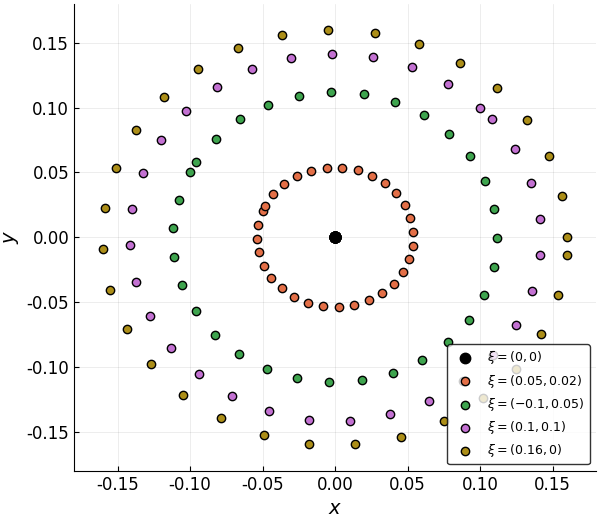
\includegraphics[width=0.8\linewidth]{euler-jt-evaluations-center}
 \caption{Transporte de jets para la ecuación \ref{eq:center} con vecindad inicial $\U_{\xo} = (0,0)^T + \xi$ usando el método de Euler en el intervalo temporal $[0,2\pi]$ en pasos de $h=10^{-4}$. Se evaluó la solución para los distintos $\xi$ marcados en la gráfica, en intervalos de $1000h$.}
 \label{fig:center-evals}
\end{figure}

Notemos que (\ref{eq:center}) es una sistema hamiltoniano cuyas soluciones en el espacio fase viven en las curvas de nivel dadas por
\begin{equation*}
H(\mathbf{x}) = \frac{1}{2} \left( x_1^2 + x_2^2 \right),
\end{equation*} 
con solución analítica
\begin{align}
 x_1(t) &= x_{01}\cos{(t)} - x_{02}\sin{(t)} \nonumber \\
 x_2(t) &= x_{01}\sin{(t)} + x_{02}\cos{(t)}.
 \label{eq:center_analytical}
\end{align}

Enla figura \ref{fig:center_anal_comparison} se muestran distintas comparaciones de la integración numérica contra las soluciones analíticas de (\ref{eq:center_analytical}).

%FIGURA! 
\begin{figure}[h!]
\centering
\begin{subfigure}{0.49\textwidth}
	\centering
	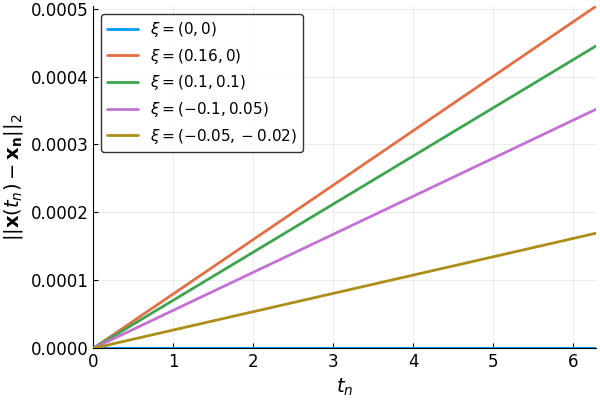
\includegraphics[width = \textwidth]{euler-vs-analytical_center}
	\caption{Norma de la diferencia entre la solución real y evaluaciones de la solución numérica para distintos valores de $\xi$ marcados en la gráfica. Se puede observar un crecimiento lineal del error numérico, lo cual es una de las consecuencias de usar el método de Euler.}
	\label{fig:center-eu_vs_anal}
\end{subfigure}
%
\begin{subfigure}{0.49\textwidth}
	\centering
	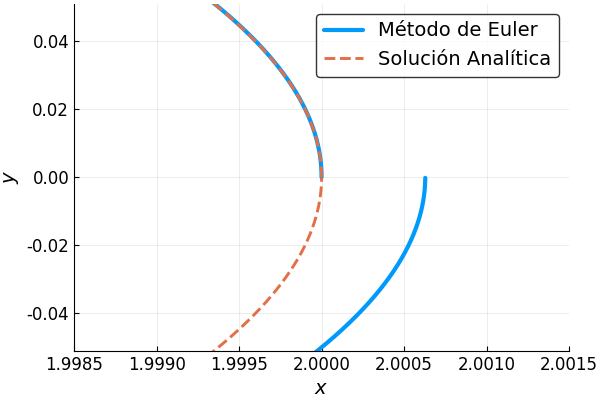
\includegraphics[width = \textwidth]{euler-method_error}
	\caption{Sección del espacio fase donde se observan la solución analítica y la solución numérica para pasos de $h=10^{-4}$ con cóndición inicial $\xo = (2,0)$. \\ \\}
	\label{fig:center_not-closed}
\end{subfigure}
\caption{Diferencias numéricas entre el método de Euler y la solución analítica para \ref{eq:center}}
\label{fig:center_anal_comparison}
\end{figure}


Queda claro que el desarrollo de TJ necesita de un álgebra polinomial para poder evaluar los distintos $P_{j,\xo}(\xi)$ que definen al campo vectorial en cada uno de sus pasos. El problema de evolucionar una vecindad $U_{\xo}$ dado un sistema dinámico $\dot{\mathbf{x}}(t) = f(t,\mathbf{x}(t))$ se reduce al problema de saber cómo se evalúan distintos polinomios en cada paso de integración, así como la definición computacional de sus operaciones. Hay muchos detalles a considerar en este problema: ¿Qué paso de integración se deberá usar para conseguir la evolución temporal de las soluciones? ¿Cómo medimos el error respecto a la solución real? ¿Existe alguna forma de controlar el error que arrojan el método de integración y la propagación de jets del TJ? ¿Cuál la complejidad de las operaciones para la aritmética de polinomios? En el apéndice \ref{chap:AlgPoli} se desarrolla el álgebra polinomial y sus operaciones tal como son implementadas en el TJ y se ahonda en esta discusión. En la sección \ref{sec:taylor-metodo} se hace el desarrollo del método de Taylor como integrador computacional adaptativo de sistemas de EDO, y en la sección \ref{sec:ind-dinam} se desarrollan distintos indicadores dinámicos utilizados en el TJ así como sencillos ejemplos ilustrativos para cada uno de ellos.

\section{Método de Taylor}
\label{sec:taylor-metodo}

Como se observa en (\ref{eq:euler}), el método de Euler es la aproximación lineal de $\mathbf{x}(t)$ con variaciones de tamaño $h$ dado. El método de Taylor es la generalización del de Euler en el sentido de que, si $\dotx = f(\mathbf{x}(t),t)$ es una función analítica, entonces $\mathbf{x}(t)$ también lo es y, por tanto, se puede expresar como una serie de potencias convergente 
\begin{equation}
\mathbf{x}(t + h) = \sum_{i=0}^\infty x_i h^i = \sum_{i=0}^\infty \frac{\mathbf{x}^{(i)}(t)}{i!}h^i 
= \sum_{i=0}^M \frac{\mathbf{x}^{(i)}(t)}{i!}h^i + \mathcal{O}(h^{M+1})
\label{eq:anal-exp}
\end{equation}
la expansión de orden $M$ en $h$ con $x_i := \mathbf{x}^{(i)}(t)$ la i-ésima derivada de $\mathbf{x}$ evaluada al tiempo $t$. En el caso que $\mathbf{x}: \mathbb{R} \to \mathbb{R}^d$, entonces $i := ||\mathbf{i}||_1 = i_1 + \cdots + i_d$ y $x_i := x_{i_1,\cdots,i_d} \in \mathbb{R}$, compactando así la notación para dimensiones $d > 1$.

Notemos que, por (\ref{eq:ode}), se define la relación de recurrencia
\begin{equation}
x_{i+1} = \frac{f_i}{i+1}
\label{eq:rec-rel}
\end{equation}

obteniendo así 
\begin{equation}
\mathbf{x}(t_{n+1}) = \mathbf{x}(t_n) + \sum_{i=1}^M f_i(\mathbf{x}(t_{n+1}),t_n)h^i + \mathcal{O}(h^{M+1})
\label{eq:taylor-rel}
\end{equation}

el \textbf{método de Taylor} para obtener $\mathbf{x}(t) = \flowci$ dado $\xo$.

Una enorme ventaja de (\ref{eq:taylor-rel}) sobre el método de Euler, o cualquier método de integración numérica con paso fijo como los Runge-Kutta, es que se puede conocer el residuo $\mathcal{O}(h^{M+1})$ en términos de $h$, controlando así el error de integración del sistema de EDO para cada paso. Como $f$ y $\mathbf{x}$ son analíticas, entonces su expansión en series de potencias es convergente. De este modo, buscamos que la contribución del último término de la serie sea menor a cierta tolerancia $\epsilon_{Taylor}$, es decir
\begin{equation*}
||x_M||_\infty h^M \leq \epsilon_{Taylor} \implies h = \left( \frac{\epsilon_{Taylor}}{||x_M||_\infty} \right)^{1/M}.
\end{equation*} 

Para el caso de funciones pares o impares, es probable que el último coeficiente de la serie sea identicamente cero y, para evitar indeterminaciones al encontrar $h$, se busca la mínima $h$ entre los dos últimos coeficientes de la expansión de $\mathbf{x}(t+h)$
\begin{equation}
h = \min_{m \in [M-1,M]}{ \left( \frac{\epsilon_{Taylor}}{||x_m||_\infty} \right)^{1/m} }
\label{eq:stepsize}
\end{equation} 
%% De acuerdo con Simo y la tesis de Dani Perez, esta no es la mejor selección para el paso de integración. De hecho, no pude demosttrar que este paso sea, en efecto, una buena elección. Sin embargo, suena como algo intuitivo ya que la serie es convergente. Ellos, sin embargo, sí acotan de manera formal la contribución del error del residuo... checarlo.

\subsection{Método de Taylor para el transporte de jets}
Para el método que se acaba de desarrollar, cada término $\mathbf{x}_i \in \mathbb{R}^d$. Sin embargo, en el TJ una vecindad $\U_{\xo}$ se parametriza con el polinomio $P_{0,\xo}(\mathbf{\xi}) \in \pkk{N}{d}$ alrededor de $\xo = \mathbf{x}(t_0)$\footnote{Consultar la sección \ref{sec:pknN} para familiarizarse con esta notación.}. Dado que $P_{0,\xo}(\mathbf{\xi}) = \U_{\xo} = \xo + \mathbf{\xi}$, la relación de recurrencia (\ref{eq:taylor-rel}) puede reescribirse como
\begin{equation}
P_{n+1,\xo}(\xi) = P_{n,\xo}(\xi) + \sum_{i=1}^M f_i(P_{n,\xo}(\xi),t_n)h^i 
\label{eq:jt-rel}
\end{equation}

donde $P_{n,\xo}(\xi) \in \pkk{N}{d} \ \forall \ n$. Así, pueden encontrarse las soluciones $\phi(t_n;t_0,\xo) = \mathbf{x}(t_n)$ con condición inicial $\xo$ y $\phi(t_n;t_0,\U_{\xo}) = P_{n,\xo}(\xi)$ la solución de la vecindad $\U_{\xo}$ al tiempo
$t_n$ del sistema (\ref{eq:ode}) usando (\ref{eq:taylor-rel}) y (\ref{eq:jt-rel}), respectivamente.

Aunque la actualización del método de Taylor para el transporte de jets es bastante directa gracias al desarrollo del álgebra polinomial, hay que prestar atención a cómo obtener el paso de integración $h$ ya que, siguiendo (\ref{eq:stepsize}), debemos tomar $||x_m||_\infty$ y para $x_m \in \pkk{N}{d}$, la p-norma no está definida.

\begin{definicion}
Sea $||\cdot|| : \mathbb{K} \to \mathbb{R}^+$, $P(\mathbf{\xi}) = \sum_{k} a_k \mathbf{\xi}^k \in \mathbb{K} = \pkk{N}{d}$. Se define la \textbf{p-norma} de $P(\xi)$ como
\begin{equation}
 ||P(\mathbf{\xi})||_p := \left( \sum_{k} ||a_k||_p^p \right)^{1/p}
 \label{eq:poly-norm}
\end{equation}  
donde, si $a_k \in \mathbb{R}$, entonces $||a_k||_p = |a_k|$.
\end{definicion}

Así, la elección del paso de integración tiene sentido ahora también para polinomios. Es importante mencionar que la definición de la norma para polinomios en $\pkk{N}{d}$ coincide con la definición estándar de norma. Además, de este modo, el paso de integración $h$ coincide por el utilizado por D. Perez en \cite{P-palau}.

\subsection{Probando el método de Taylor}
\label{sec:benchmark-taylor}

Es hora de empezar a poner las manos en la masa y ver si, en efecto, los métodos planteados en (\ref{eq:taylor-rel}) y (\ref{eq:jt-rel}) son suficientemente precisos para dejar nuestra conciencia tranquila. 

Tomaremos, a manera de ejemplo, un par de \textbf{sistemas hamiltonianos} de la forma
\begin{equation}
 H(\mathbf{p},\mathbf{q}) = \frac{1}{2m}\mathbf{p}^2 + V(\mathbf{q})
 \label{eq:hamiltonian}
\end{equation}
%V = V(p,q) ? 

donde $H: \mathbb{R}^{3N}\times\mathbb{R}^{3N} \to \mathbb{R}$ es el hamiltoniano del sistema y representa la energía, con $N$ la dimensionalidad del espacio. $H$ es una primera integral del sistema
\begin{align}
 \dot{\mathbf{p}} &= -\frac{\partial{H}}{\partial{\mathbf{q}}} \nonumber \\
 \dot{\mathbf{q}} &= \frac{\partial{H}}{\partial{\mathbf{p}}}
\label{eq:ham-rel}
\end{align}

y su primera integral (\ref{eq:hamiltonian}) representa una constante de movimiento que, físicamente, representa la conservación de la energía total.

Así, comprobar los métodos de integración para sistemas conservativos como (\ref{eq:hamiltonian}) será comparar la energía para cada paso temporal dado en relación a la energía inicial, lo cual debería ser constante. 
Dado que conozcamos la solución analítica de algún sistema, se puede comparar dicha solución contra la calculada por los diferentes métodos de integración.

\subsubsection{Oscilador armónico}
\label{sec:oscilador}
Sea un sistema dado por una masa $m$ que, al desplazarlo de su estado de equilibrio por una cantidad $\mathbf{x}$, siente una fuerza restitutiva proporcional a dicho desplazamiento
\begin{equation}
 \mathbf{F}(\mathbf{x}) = m \ddot{\mathbf{x}} = - k\mathbf{x}
 \label{eq:oscilador_force}
\end{equation}
con $[k] = \frac{Kg}{s^2}$  y $k>0$. 

Tomando $\mathbf{v} = \dot{\mathbf{x}}$ se obtiene
\begin{align}
 \dot{\mathbf{x}} &= \frac{k}{m} \mathbf{p} \nonumber \\
 \dot{\mathbf{v}} &= - \frac{k}{m} \mathbf{x}
 \label{eq:oscilador_ode}
\end{align}
las EDO para el \textbf{oscilador armónico}, las cuales son equivalentes, para $\omega^2 := \frac{k}{m} = 1$ y $\mathbf{x} \in \mathbb{R},\ \mathbf{p} \in \mathbb{R}$, a (\ref{eq:center}). 

La primera integral de (\ref{eq:oscilador_ode})
\begin{equation}
 H(\mathbf{p},\mathbf{x}) = \frac{1}{2m}p^2 + \frac{\omega^2}{2} x^2
 \label{eq:oscilador_ham}
\end{equation}
con $p=mv$, cumple con las ecuaciones de (\ref{eq:ham-rel}), una constante de movimiento que representa la energía.

%FIGURA!
\begin{figure}[h!]
 \centering
 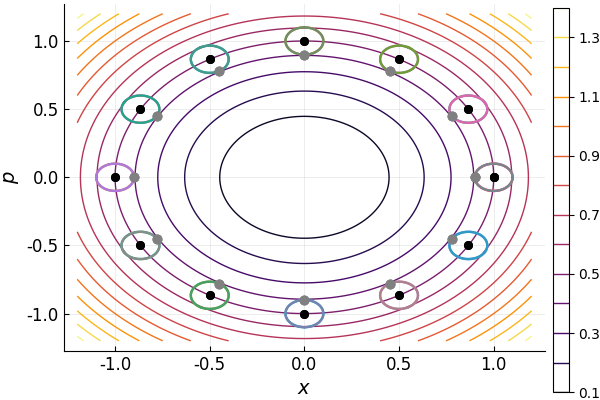
\includegraphics[width=0.8\linewidth]{oscillator_phsp}
 \caption{Se utilizó tolerancia $\epsilon_{Taylor} = 10^{-20}$ y orden de la expansión $M = 28$.}
 \label{fig:oscilador_phsp}
\end{figure}

Así, tenemos que las soluciones analíticas son de la forma 
\begin{align}
 x(t) &= v_{0}\sin{(\omega t)} + x_{0}\cos{(\omega t)} \nonumber \\ 
 v(t) &= v_{0}\omega\cos{(\omega t)} - x_{0}\omega\sin{(\omega t)}. 
 \label{eq:oscilador_analytical}
\end{align}

La figura \ref{fig:oscilador_phsp} presenta al espacio fase del oscilador armónico, junto con una solución calculada con el transporte de jets. En ésta se observa cómo las soluciones evaluadas en una vecindad inicial parametrizada por un círculo están siempre en las líneas de las curvas de nivel del hamiltoniano. Se observa además en la figura la estructura de centros alrededor del único punto singular $(0,0)^T$.

Dada la condición inicial $\xo = (1,0)^T$ y tomando $m = 1 \ Kg$, $k = 1 \frac{Kg}{s^2}$, tenemos que el oscilador con energía total de $E_0 = H(\xo) = 1$ Joule. En la figura \ref{fig:} se pueden ver las variaciones $\delta E$ de la energía en cada paso de integración así como la diferencia $\delta \mathbf{x}$ de las soluciones de jet calculadas por el método de Taylor evaluadas en diferentes $\xi$s y las soluciones analíticas del oscilador armónico correspondientes al desplazamiento dado por las $\xi$s.

%FIGURA!
 \begin{figure}[h!]
\centering
\begin{subfigure}{0.49\textwidth}
	\centering
	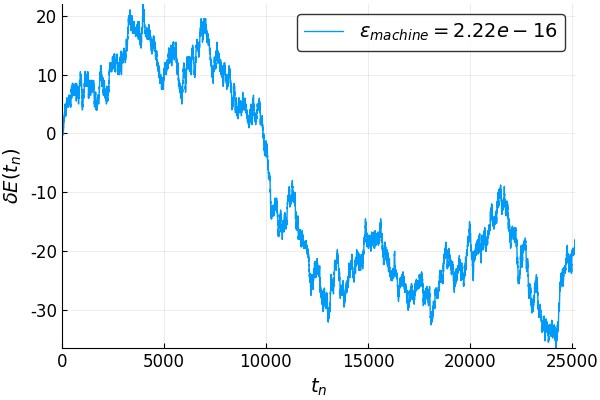
\includegraphics[width = \textwidth]{oscillator_dE}
	\caption{}
	\label{fig:pendulum_jt_O1}
\end{subfigure}
%
\begin{subfigure}{0.49\textwidth}
	\centering
	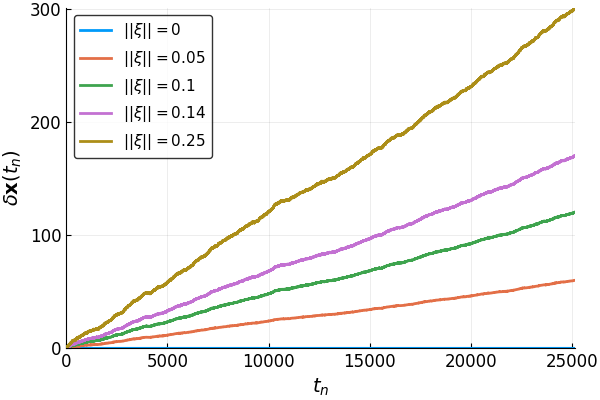
\includegraphics[width = \textwidth]{oscillator_dx}
	\caption{}
	\label{fig:pendulum_jt_O4}
\end{subfigure}
\caption{Se utilizó tolerancia $\epsilon_{Taylor} = 10^{-20}$ y orden de la expansión $M = 28$.}
\label{fig:pendulum_jt}
\end{figure}

\cleardoublepage
\subsubsection{Péndulo simple}
\label{sec:pendulo}
Sea un sistema donde una masa $m$ está anclada al extremo de una varilla de longitud $l$ cuya masa es despreciable. Esta varilla está anclada, a su vez, a un punto inmovil. Así, $m$ se mueve bajo la acción de la gravedad $\mathbf{g}$ como se muestra en la figura \ref{fig:pendulo}, ignorando la resistencia del aire.

%FIGURA! 


La forma más natural de trabajar este problema es en coordenadas polares, en donde la masa $m$ se mueve con una velocidad $v = l\dot{\theta}$ con $l$ constante, es decir $r = l \neq r(t) \implies \dot{r} = \dot{p_r} = 0$. Esta constricción reduce en uno los grados de libertad del sistema, haciendo que éste dependa únicamente de $\theta$. 

Tenemos que 
\begin{align}
 K &= \frac{1}{2}m v^2 = \frac{1}{2} m l^2 \dot{\theta}^2 \nonumber \\
 U &= mgh(\theta) = mgl\left(1 - \cos{\theta} \right)
\end{align}
son la energía cinética y potencial, respectivamente. 

Así, contruimos el lagranjiano del sistema
\begin{equation*}
 \mathcal{L}(\theta,\dot{\theta}) = K - U = \frac{1}{2} m l^2 \dot{\theta}^2 - mgl\left(1 - \cos{\theta} \right).
\end{equation*}
Sabemos, por (\ref{eq:lagr-ham-rel}), que
\begin{equation*}
 \mathbf{p} = \frac{\partial \mathcal{L}}{\partial \mathbf{\dot{q}}} = ml^2\dot{\theta}
\end{equation*}

obteniendo la coordenada conjugada de momento y, así, plantear el hamiltoniano, o energía total del sistema, como
\begin{equation}
 H(p,\theta) = K + U = \frac{p_{\theta}^2}{2ml^2} + mgl\left(1 - \cos{\theta} \right).
\label{eq:pendulo-ham}
\end{equation}
 
Las EDO quedan entonces, por (\ref{eq:ham-rel}), como
\begin{align}
 \dot{\theta} &= \frac{p_{\theta}}{ml^2} \nonumber \\
 \dot{p_{\theta}} &= -mgl\sin{\theta} 
\label{eq:pendulo-ode}
\end{align}

en cuyo dominio $(\theta,p_{\theta}) \in [-\pi,\pi]\times[p_{min},p_{max}] \subset \mathbb{R}^2$ existen tres puntos singulares: $(-\pi,0),(\pi,0), (0,0)$; dos puntos de ``liberación'' y otro de ``relajación'', respectivamente. En la figura \ref{fig:pendulum_pshp} se puede ver una representación del espacio fase donde se exhibe el comportamiento de dichos puntos.

%FIGURA!
\begin{figure}[h!]
 \centering
 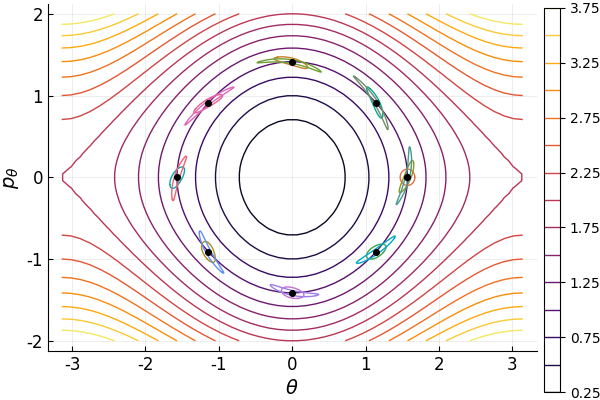
\includegraphics[width=0.8\linewidth]{pendulum_phsp}
 \caption{Espacio fase para el péndulo simple representado por la ecuación \ref{eq:pendulo-ham}. En negro salen puntos de la trayectoria calculada con el método de Taylor para Jets con $\xo = (\frac{\pi}{2},0)^T$, tolerancia $\epsilon_{Taylor} = 10^{-20}$, orden de la expansión $M = 28$ y sus vecindades (jets) evaluadas para $\mathbf{\xi}(\tau) = 0.1\cdot \left( \cos(\tau), \sin(\tau) \right)^T$, $\tau \in [0,1]$.}
\label{fig:pendulum_pshp}
\end{figure}

Si viajamos a un planeta en donde $g = 1 \ \frac{m}{s^2}$ \footnote{A veces, para la física, es más fácil viajar a un planeta donde exista la atracción gravitacional que más nos gusta que hacer a un péndulo girar en la Tierra; qué comodo.} y tomamos una varilla de longitud $l=1$ m y una masa $m=1$ kg,  entonces, para las condiciones iniciales $p_{\theta}(0) = 0 \ N \cdot m$ y $\theta(0) = \pi/2$, la energía total es 
\begin{equation*}
E_0 = H(p_{\theta}(0),\theta (0) ) = 1 \text{ J.}
\end{equation*}

Para dichas condiciones, se puede integrar el transporte de jets y además, evaluarlo para condiciones cercanas y ver cómo se comportan éstas soluciones en el espacio fase, que deben, en teoría, moverse por las curvas de (\ref{eq:pendulo-ham}). Se puede observar de la figura \ref{fig:pendulum_jt} cómo para jets de orden 4, las soluciones se quedan sobre las curvas de nivel del hamiltoniano.

%FIGURA!
\begin{figure}[h!]
\centering
\begin{subfigure}{0.49\textwidth}
	\centering
	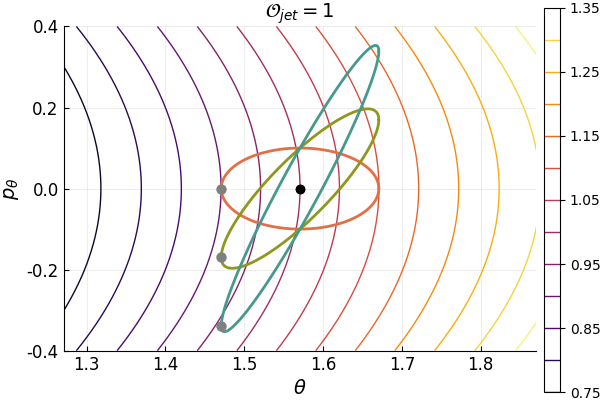
\includegraphics[width = \textwidth]{pendulum_jt_O1}
	\caption{Jet de orden $1$ después de dos periodos desde $\xo$.}
	\label{fig:pendulum_jt_O1}
\end{subfigure}
%
\begin{subfigure}{0.49\textwidth}
	\centering
	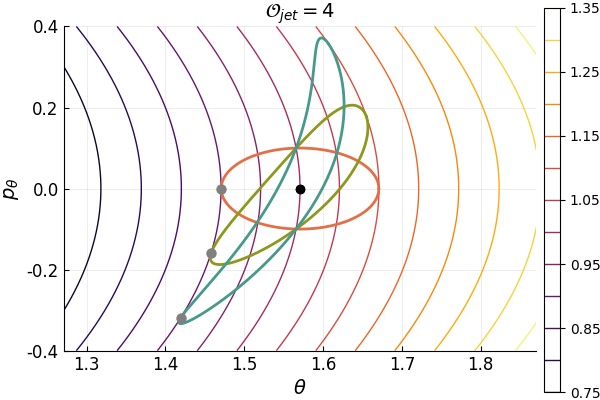
\includegraphics[width = \textwidth]{pendulum_jt_O4}
	\caption{Jet de orden $4$ después de dos periodos desde $\xo$.}
	\label{fig:pendulum_jt_O4}
\end{subfigure}
\caption{Jets de distinto orden para $\U_{\xo}$ parametrizada en un círculo de radio 0.1 $\mathbf{\xi}(\tau) = 0.1\left( \cos(\tau),\sin(\tau) \right)^T$ alrededor de $\xo = (\frac{\pi}{2},0)^T$ en el péndulo simple. Se utilizó tolerancia $\epsilon_{Taylor} = 10^{-20}$ y orden de la expansión $M = 28$.}
\label{fig:pendulum_jt}
\end{figure}

Respecto a las variaciones de energía en el sistema, se ve en la figura \ref{fig:pendulum_dE} cómo $\delta E(t)$ varía alrededor de cero como un movimiento browniano. Éste último se relaciona con los errores de redondeo de puntos flotantes de la máquina y no con el método de Taylor en sí, a diferencia del método de Euler, como se observa en la figura \ref{fig:center_anal_comparison}, donde el error crece de manera lineal. La máxima variación respecto a la energía inicial es de $2.28\times10^{-14}$, lo cual corresponde a $103 \epsilon_{machine}$ (sin redondear).

%FIGURA! 
\begin{figure}[h!]
 \centering
 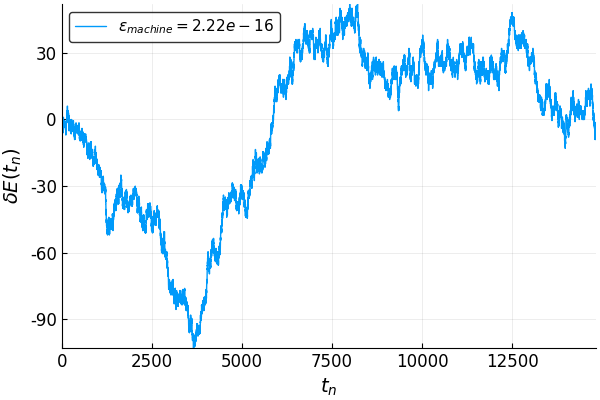
\includegraphics[width=0.8\linewidth]{pendulum_dE}
 \caption{Diferencia $\delta E(t_n) := \frac{E(t_n) - E_0}{\epsilon_{machine}}$ de la energía del péndulo simple con condición inicial $\xo = (\frac{\pi}{2},0)$, tolerancia $\epsilon_{Taylor} = 10^{-20}$ y orden de la expansión $M = 28$.}
 \label{fig:pendulum_dE}
\end{figure}

\subsubsection{Péndulo periódicamente forzado}


\section{Indicadores dinámicos de campos vectoriales con base en el transporte de jet}
\label{sec:ind-dinam}

%choro

\subsection{Tamaño máximo de las vecindades}